\chapter{UPMEM}
%\label{chapter:title}

\section{The company}

UPMEM is a fabless semiconductor company. It was founded in 2015 by electronics engineers Gilles Hamou and Fabrice Devaux.

At the time of this writing it counts nineteen employees, mostly located at the Grenoble office. There is a secondary office at Station F in Paris, and a couple of employees work remotely.

\section{The product}
UPMEM's main product is a memory-centric hardware accelerator for data-intensive applications, generally referred to as PIM, for Processing-in-Memory. It is sold either as individual memory sticks (DIMM), or preinstalled in an Intel server. The company also offers PIM-enabled cloud computing services for customers and researchers.

UPMEM PIM boasts the following features:

\begin{itemize}
    \item \textbf{General-purpose processor:} A wide range of instruction set for various types of calculation.
    \item \textbf{Massively parallel:} Up to 2560 PIM units can be combined in a single socket server with 256GB PIM DRAM.
    \item \textbf{Larger bandwidth:} 2,5 Tera bytes per second of memory bandwidth.
    \item \textbf{Extra computing power:} Roughly equivalent to 15 additional x86, with the main CPU used for orchestration.
\end{itemize}

So far some of the most mature and successful applications are:

\begin{itemize}
    \item \textbf{UPVC:} A genomic application for mapping and variant calling.
    \item \textbf{Index Search:} A database application.
\end{itemize}

Most of the applications so far are however at the prototype stage.

\section{The team}
I was attached to the Application and SDK team for my apprenticeship, under the supervision of tech lead Julien Legriel. The team is part of the software department, headed by director Denis Makoshenko.

There are five members in the Application and SDK team: the tech lead, two software engineers, one CIFRE PhD candidate and myself.

\subsection{Work environment}
\begin{itemize}
    \item \textbf{OS:} All software employees work in a Linux environment (Ubuntu Budgie in my case).
    \item \textbf{Machines:} There are several PIM-enabled cloud servers reserved for development and internal R\&D, accessible via a SSH connection. There are also regular servers for development and CI accessible only through the company LAN. Server access and security is provided by JumpCloud services. All servers and cloud machines run on Debian.
    \item \textbf{Sources:} The UPMEM toolchain source code is hosted on private GitHub repositories. It is tested nightly on a local server with Jenkins. The applications codes are also hosted on the company GitHub account, with visibility settings depending on the project confidentiality.
    \item \textbf{Cloud:} When the need arises for extra computing power or for GPU calculations, the company subscription to AWS allows me to use EC2 instances. For long-term storage, the company uses a Google Drive.
    \item \textbf{Project tracking:} The company uses Jira for project tracking, although this is a recent addition, and most workflows are not yet integrated.
\end{itemize}

This template aims to simplify and improve the (Xe)LaTeX report template by EPFL. Some of the main features:

\begin{itemize}
  \item \textbf{Simplicity First:} A class file that has been reduced by nearly 70\% to simplify customization;
  \item \textbf{Effortless:} Many common packages are included to get started immediately;
  \item \textbf{Complete:} Ready-to-go when it comes to document and file structure.
\end{itemize}

\noindent This template works with pdfLaTeX, XeLaTeX and LuaLaTeX. In order to adhere to the EPFL house style, either XeLaTeX or LuaLaTeX is required, as it supports TrueType and OpenType fonts. BibLaTeX is used for the bibliography with as backend biber. Please visit \url{https://batuhanfaik.github.io/report} for the full documentation.

\begin{figure}[h]
    \centering
    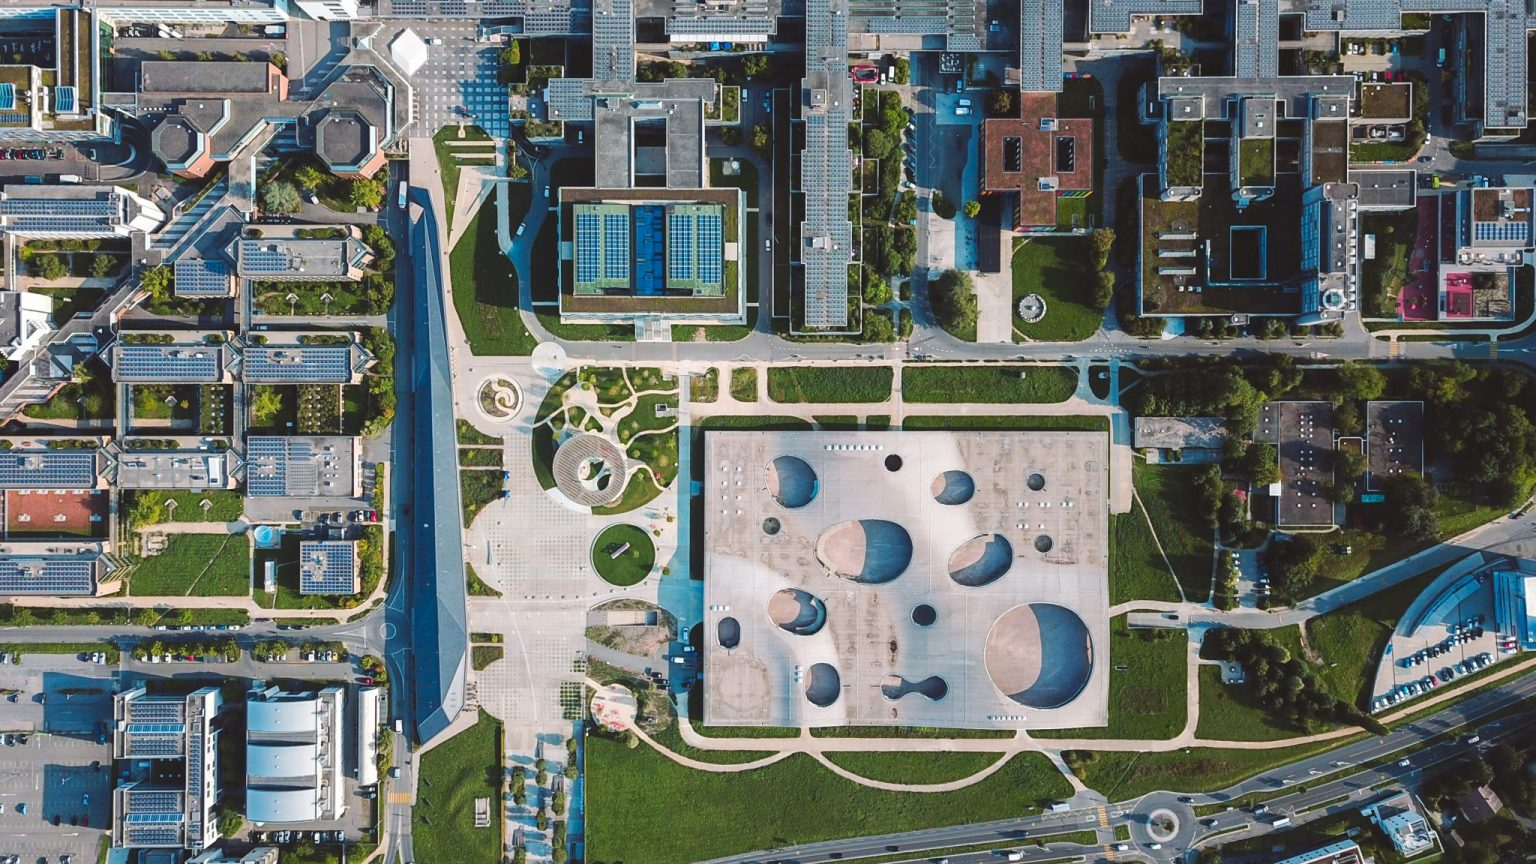
\includegraphics[width=0.95\linewidth]{figures/campus.jpg}
    \caption{EPFL Campus}
\end{figure}

\section*{License}

\noindent This template is available under CC BY-NC 4.0. For more information, see \url{https://creativecommons.org/licenses/by-nc/4.0/}. No attribution is required in reports created using this template.
